\documentclass[border=10pt]{standalone}
%%%<
\usepackage{verbatim}
%%%>
\usepackage{pgfplots}
\pgfplotsset{width=7cm,compat=1.8}
\begin{comment}
:Title: Constant plot
:Tags: 2D;Constant plots;Manual
:Author: Christian Feuersänger
:Slug: constant-plot

Constant plots draw lines parallel to the x-axis to connect coordinates. The
discontinuous edges may be drawn or not, and marks may be placed on left or
right ends.

The code is from the PGFPlots 1.10 manual: "4.5.3 Constant Plots".
\end{comment}
\begin{document}
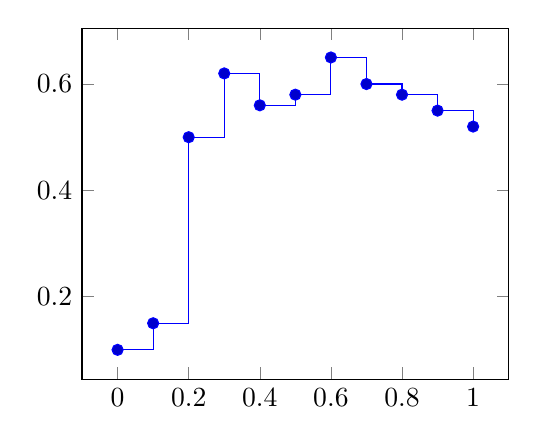
\begin{tikzpicture}
  \begin{axis}
    \addplot+[const plot]
      coordinates
        {(0,0.1) (0.1,0.15) (0.2,0.5) (0.3,0.62)
         (0.4,0.56) (0.5,0.58) (0.6,0.65) (0.7,0.6)
         (0.8,0.58) (0.9,0.55) (1,0.52)};
  \end{axis}
\end{tikzpicture}
\end{document}
